\chapter{Theory}
\label{chap:theory}
Earnshaw's theorem says that it is impossible to achieve stable levitation of a non-diamagnetic object using static fields alone. The reason for this is that the magnetic potential cannot have minima but only saddle points. This means that the tiniest perturbation will cause the object to fall. One way to circumvent this is to use superconductors which are diamagnetic or to use dynamic fields. A magnetic Paul trap uses the latter. This chapter will outline the relevant theory and design considerations for a magnetic Paul trap.

\section{Magnetic levitation}
\label{sec:magnetic_levitation}
The energy of a magnetic object in a magnetic field is given by:
\begin{equation}
    E = -\vec{\mu} \cdot \vec{B}
    \tag{magnetic potential}
    \label{eq:magnetic_potential_definition}
\end{equation}
where $\vec{\mu}$ is the magnetic moment of the object and $\vec{B}$ is the magnetic field. A magnetic Paul trap uses a static homogeneous field ($\vec{B_0}$) to align the magnetic moment of the object. In our case we assume alignment with the $z$-axis. A second dynamic field ($\vec{B_1}$) contains the saddle point. Because the field is dynamic, the unstable direction is time dependent. By rapidly changing the field, the object is effectively trapped in the saddle point. This leads to a ponderomotive force\cite{perdriat}. Finally a gradient field ($\vec{B_2}$) is used to counteract the gravitational force\cite{perdriat}. In the remainder of this section we will derive the magnetic potential and the associated eigenfrequencies.

\subsection{Fields}
\label{subsec:fields}
The homogeneous field is given in \autoref{eq:homogeneous_field}. It too is oriented in the $z$-axis with magnitude $B_0$. In our experiment we will use two Helmholtz coils to create this field.
\begin{equation}
    \vec{B_0}(\vec{r}, t) = \vec{B_0} = B_0 \zhat
    \label{eq:homogeneous_field}
\end{equation}

The static field is given in \autoref{eq:saddle_point}. $B_1''$ is the curvature of $\vec{B_1}$ and $\Omega / 2\pi$ the frequency of the oscillation. The field is created using two coplanar loops of with a current in opposite directions. These loops are the main focus of this thesis. Given the radius of the inner (outer) loop $r_1$ ($r_2$) we can express the curvature as $B_1'' = -\frac{9}{16}\mu_0i_1/r_1^3$ where $i_1$ ($i_2$) is the current through the inner (outer) loop\cite{perdriat}. This assume that $i_2/i_1 = -r_2/r_1 = -\xi$.
\begin{equation}
    \vec{B_1}(\vec{r}, t) = \frac{B_1''}{2} \begin{pmatrix}
        -xz \\
        +yz \\
        z^2 - \frac{1}{2}\left(x^2 + y^2\right)
    \end{pmatrix} \cos(\Omega t)
    \label{eq:saddle_point}
\end{equation}

Finally we have the gradient field, given in \autoref{eq:gradient_field}. The required gradient can be expressed as $B_2' = mg/\mu$ where $m$ is the mass of the levitated object, $g$ the gravitational acceleration and $\mu$ the magnetic moment of the object. The gradient serves to offset the effect of gravity. As such the gradient is also oriented in the $z$-axis. The gradient field can be created by using a larger current in one of the Helmholtz coils.
\begin{equation}
    \vec{B_2}(\vec{r}, t) = B_2' \begin{pmatrix}
        -x / 2 \\
        -y / 2 \\
        z
    \end{pmatrix}
    \label{eq:gradient_field}
\end{equation}

\subsection{Magnetic potential}
\label{subsec:magnetic_moment}
Using the $zyz$ convention for the Euler angles ($\alpha$, $\beta$, $\gamma$) we can express the magnetic moment as in \autoref{eq:magnetic_moment}\cite{perdriat}. In this equation $\tilde\beta = \beta - \pi/2$.
\begin{equation}
    \vec{\mu} = -\mu \begin{pmatrix}
        -\cos(\alpha)\sin(\tilde\beta)\cos(\gamma) - \sin(\alpha)\sin(\gamma) \\
        \cos(\alpha)\sin(\gamma) - \sin(\alpha)\sin(\tilde\beta)\cos(\gamma) \\
        -\cos(\tilde\beta)\cos(\gamma)
    \end{pmatrix}
    \label{eq:magnetic_moment}
\end{equation}

By taking the inner product of the magnetic moment and the fields we can derive the magnetic potential. This is given in \autoref{eq:magnetic_potential}. The potential is a function of the position of the object $\vec{r}$ and the orientation of the magnetic moment $\vec{\mu}$\cite{perdriat}.
\begin{equation}
    E_\text{mag}(\vec{r}, \vec{\mu}) = \mu B_0 \left(\frac{\gamma^2}{2} + \frac{\tilde\beta^2}{2}\right) - \frac{\mu B_1''}{2} \left(z^2 - \frac{1}{2}\left(x^2 + y^2\right)\right)\cos(\Omega t)
    \label{eq:magnetic_potential}
\end{equation}

\subsection{Eigenfrequencies}
\label{subsec:eigenfrequencies}
Starting from \autoref{eq:magnetic_potential} and averaging over the oscillation period we can derive the eigenfrequencies\cite{perdriat}. They are given in \autoref{eq:eigenfrequencies}. In these equations $a$ is the radius of the levitated object (such that $V \sim a^3$) and $\rho_m$ is the density of the object. The eigenfrequencies associated with the orientation of the magnet depend on $B_0$, which intuitively makes sense since the orientation of the magnet is determined by the homogenous field. The eigenfrequencies associated with the position of the magnet depend on $B_1''$, which also makes sense since the alternating field is what restricts the movement of the object.
\begin{equation}
    \begin{gathered}
        \omega_\gamma = \omega_{\beta} = \sqrt{\frac{5}{2}\frac{B_0B_\text{sat}}{\mu_0 \rho_m a^2}} \\
        \omega_z = 2\omega_x = 2\omega_y = \frac{\Omega \abs{q_z}}{2\sqrt{2}} = \frac{1}{\sqrt{2}}\frac{B_1''B_\text{sat}}{\mu_0\rho_m\Omega}
    \end{gathered}
    \label{eq:eigenfrequencies}
\end{equation}

The time average is valid if $q_z$, as defined in equation \ref{eq:frequency-constraint}, is less than or equal to $0.4$\cite{perdriat}.
\begin{equation}
    q_z = -2q_x = -2q_y = \frac{2}{\Omega^2}\frac{B_1''B_{\text{sat}}}{\mu_0\rho_m}
    \label{eq:frequency-constraint}
\end{equation}

Rotation around the $z$-axis (the angle $\alpha$) is not restricted by any magnetic field. This is because of the spherical symmetry in the system around the $z$-axis. If we assume that the object is in thermal equilibrium then we can estimate the angular frequency:
\begin{equation}
    I\omega_\alpha^2 \approx k_B T \Rightarrow \omega_\alpha \approx \sqrt{\frac{k_B T}{I}} = \sqrt{\frac{15 k_B T}{8 \pi \rho_m a^5}}
\end{equation}
In this equation $I$ is the moment of inertia of the object. The moment of inertia of a sphere is given by $I = \frac{2}{5} m a^2$. Due to the spherical symmetry of the object this mode is very hard to detect experimentally.

In short, the eigenfrequencies are determined by the magnetic fields and the size of the object. The orientation of the magnetic moment and the associated librational eigenfrequencies are determined by the homogenous field. The position of the object and the associated vibrational eigenfrequencies are determined by the dynamic field. The rotation around the $z$-axis of the object is not restricted by any magnetic field.


\section{Damping}
\label{sec:damping}
Most physical systems are damped (dissipative). In the case of a magnetic Paul trap we mostly consider three sources of damping: gas damping, inductive damping and eddy current damping. They are discussed in the remainder of this section. For an excellent review of relevant damping mechanisms see \citeauthor{millen}. The resonance peak of a damped harmonic oscillator has a finite width and height related to the quality factor $Q$. The quality factor is defined as the ratio of the energy stored in the system to the energy dissipated per cycle. We define the Q-factor as follows:
\begin{equation*}
    Q = \omega_0 \frac{\text{energy stored}}{\text{dissipation}} = \frac{\omega_0}{\gamma}
\end{equation*}
where $\omega_0$ is the resonance frequency and $\gamma$ the damping rate. More information on the definition and conversion of Q-factors can be found in Appendix~\ref{app:q_factors}.

\subsubsection{Gas damping}
\label{subsubsec:gas-damping}
Gas damping on levitated micrometer sized particles has been studied by \citeauthor{millen}. For pressures above \qty{1E-6}{\milli\bar} and $K_n \ll 1$ stachastic forces dominate the damping rate. The damping rate in this case is given by \autoref{eqn:gas-damping-rate}.

\begin{equation}
    \frac{\gamma_{\text {gas}}}{2 \pi}=3 \mu_v \frac{a}{m} \frac{0.619}{0.619+K_n} \left( 1+c_K \right)
    \label{eqn:gas-damping-rate}
\end{equation}

$K_n$ is the Knudsen number defined as $K_n = \bar{l}/a$, $\bar{l}$ the mean free path of air molecules, $\mu_v$ the gas viscosity, $a$ the diameter of the particle, $m$ the mass of the particle and the constant $c_K = 0.31 K_n / \left(0.785 + 1.152 K_n + K_n^2 \right)$. An estimate for the gas damping as function of pressure is shown in \autoref{fig:gas-damping}.

\begin{SCfigure}
    \centering
    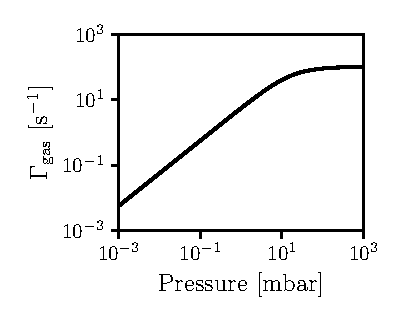
\includegraphics{figures/data/gas_damping.pdf}
    \caption{The gas damping predicted for our particle. The damping rate is calculated using \autoref{eqn:gas-damping-rate}. The calculations have been performed for $T=\qty{300}{\kelvin}$.}
    \label{fig:gas-damping}
\end{SCfigure}

\subsubsection{Inductive damping}
\label{subsubsec:inductive-damping}
The enclosed flux in the loops will change as the particle moves. A changing flux induces a current in the loops which is a dissipative process. Using COMSOL we make an estimate of the dissipation by calculating the induced current in the loops.

TODO: we still need to do this simulation, but I think it will be very similar to the Eddy current damping? Need to check what COMSOL does exactly.

\subsubsection{Eddy current damping}
\label{subsubsec:eddy-current-damping}
Eddy currents are small `whirlpools' of current that are induced by a changing magnetic field. Due to the resistance of the conductor this will lead to dissipation of energy.
TODO: add more information on this.
